% !TeX encoding = windows-1251
%& -shell-escape
\documentclass[10pt]{article}
\usepackage{newlistok}
\usepackage{tikz,ifthen}
%\usepackage[bookmarks=false, colorlinks, unicode, pdfstartview=FitH]{hyperref}
\usetikzlibrary{calc}
\pagestyle{plain}

\УвеличитьШирину{1cm}
\УвеличитьВысоту{.5cm}

\sloppy

\newcommand{\tw}[1]{\texttt{#1}} % TypeWriter

\newcommand{\skipcol}{\qquad\qquad\qquad}
\newcommand{\rulez}{\rule[-12pt]{0pt}{29pt}}
\newcommand{\rulezz}{\rule[-13pt]{0pt}{31pt}}

\title{Документация к стилевому пакету \texttt{newlistok.sty}}
\date{Версия пакетов 5.01b, последнее обновление: \сегодня~г.}


\def\BeforeTitle{\vspace{1\baselineskip}\par\noindent}
\def\AddTitleToContents{}


\begin{document}


\maketitle


\tableofcontents
\pagebreak





\section{Общие сведения}

\subsection{История}
Пакет создан на основе стиля В.Крюкова (часть синтаксиса), используя некоторые идеи стиля Городенцева
(автоматическая генерация кондуитов), а также сокращения стиля DMVN corp. Для русификации используются разработки Львовского. Кроме того, документация части стиля, скопированной со стиля DMVN corp., также скопирована с документации к стилю DMVN. О DMVN можно узнать на \verb'http:\\www.dmvn.mexmat.ru'

\subsection{Зависимости от других пакетов}
%Для работы пакета необходим пакет-русификация \texttt{russ.sty} (к пакету прилагается)

Пакет используют несколько стандартных пакетов: \texttt{inputenc}, \texttt{amssymb},
\texttt{amsmath}. Все они входят в~полный комплект \TeX{} (например, в пакет
MiK\TeX, который можно скачать из~архивов CTAN).

Подключать пакет \tw{babel} при использовании \tw{newlistok.sty} не нужно.
Компилировать файлы надо командой \tw{latex}, \tw{texify}, а ещё лучше \tw{PDFlatex} или \tw{PDFTexify}.



\subsection{Подключение и опции}
Для использования всех возможностей достаточно подключить только пакет \texttt{newlistok.sty},
все остальные будут подключены автоматически. В~стандартной ситуации основной документ
в~преамбуле может содержать только одну строку:
\begin{verbatim}
\usepackage{newlistok}
\end{verbatim}

У пакета \texttt{newlistok.sty} есть несколько модификаторов оформления: \verb'vmsh/exam/school/algerba/geometry'.
Они несколько модифицирую оформление задач, заголовков и т.д.
Подробнее об этом будет ниже.
По умолчанию установлена опция \texttt{school}.

% Пакет \texttt{newlistok.sty} имеет опцию: \verb'vmsh/exam/school/algerba/geometry'. Они работают как переключатели и~означают следующее:
% \ctab{|c|c|}{
% \hline \texttt{vmsh/exam/school/algerba/geometry} & Стиль для ВМШ/собеседований/листочков/алгебры/геометрии\\
% \hline}


Опции устанавливаются обычным образом при подключении пакета, например:
\begin{verbatim}
\usepackage[exam]{newlisok}
\end{verbatim}

Кроме того, существует возможность произвольного масштабирования. Для этого пишем
\begin{verbatim}
\usepackage[mag=930]{newlisok}
\end{verbatim}
Где вместо 930 можно поставить своё число.
Это позволяет уместить на страницу необходимый объём задач, при этом оставив шрифт как можно крупнее.

%\pagebreak

\newpage
\section{Типичный листок}
\thispagestyle{empty}
Начнём с самого простого примера. Исходный код типичного листочка будет выглядеть так:
\begin{verbatim}
\documentclass[12pt]{article}
\usepackage{newlistok}

\Заголовок{Предел последовательности\т 2}
\НомерЛистка{18}
\ДатаЛистка{12.2013}

\begin{document}
\СоздатьЗаголовок

\ввзадача[Теорема Вейерштрасса]
Докажите, что любая ограниченная монотонная последовательность сходится.
\кзадача

\задача
Докажите, что существует предел...
\кзадача

\опр
\label{Acc1}
Число~$a$ называется \emph{предельной точкой} последовательности~$(x_n)$,
если для всякого числа $\ep>0$ и~для любого $k\in\N$
существует такое натуральное $n>k$, что выполняется неравенство $|x_n-a|<\ep$.
\копр

\опр
\label{Acc2}
Точка~$a$ называется {\it предельной точкой} последовательности~$(x_n)$,
если любая окрестность точки~$a$ содержит бесконечно много точек последовательности~$(x_n)$.
\копр

\задача
Докажите эквивалентность определений~\ref{Acc1} и~\ref{Acc2}.
\кзадача

\задача
\пункт
Докажите, что если последовательность имеет предел, то этот предел является
предельной точкой и~других предельных точек нет.\\
\пункт
Верно ли, что если последовательность имеет единственную предельную точку,
то она (последовательность) является сходящейся?
\кзадача

\ввзадача[Критерий Коши]
\пункт Докажите, что сходящаяся последовательность является фундаментальной;
\пункт Докажите, что фундаментальная последовательность имеет предел.
\кзадача

\ЛичныйКондуит{0mm}{6mm}

\end{document}
\end{verbatim}
\bigskip
Результат такого кода можно увидеть на следующей странице:
\newpage
\fontsize{12}{14}\selectfont
\thispagestyle{empty}
\Заголовок{Предел последовательности\т 2}
\НомерЛистка{18}
\ДатаЛистка{12.2013}
\СоздатьЗаголовок

\ввзадача[Теорема Вейерштрасса]
Докажите, что любая ограниченная монотонная последовательность сходится.
\кзадача

\задача
Докажите, что существует предел...
\кзадача

\опр
\label{Acc1}
Число~$a$ называется \emph{предельной точкой} последовательности~$(x_n)$, если для всякого числа $\ep>0$ и~для любого $k\in\N$ существует такое натуральное $n>k$, что выполняется неравенство $|x_n-a|<\ep$.
\копр

\опр
\label{Acc2}
Точка~$a$ называется {\it предельной точкой} последовательности~$(x_n)$, если любая окрестность точки~$a$ содержит бесконечно много точек последовательности~$(x_n)$.
\копр

\задача
Докажите эквивалентность определений~\ref{Acc1} и~\ref{Acc2}.
\кзадача

\задача
\пункт
Докажите, что если последовательность имеет предел, то этот предел является предельной точкой и~других предельных точек нет.\\
\пункт
Верно ли, что если последовательность имеет единственную предельную точку, то она (последовательность) является сходящейся?
\кзадача

\ввзадача[Критерий Коши]
\пункт Докажите, что сходящаяся последовательность является фундаментальной;
\пункт Докажите, что фундаментальная последовательность имеет предел.
\кзадача

\ЛичныйКондуит{0mm}{6mm}
\ОбнулитьКондуит
\newpage
\fontsize{11}{13}\selectfont

Если вам не нравится русский язык в командах, то нет проблем:

\begin{verbatim}
\documentclass[12pt]{article}
\usepackage{newlistok}

\ListTitle{Предел последовательности\т 2}
\ListNumber{18}
\ListDate{\mmyy}

\begin{document}
\CreateTitle

\begin{iiproblem}[Теорема Вейерштрасса]
Докажите, что любая ограниченная монотонная последовательность сходится.
\end{iiproblem}

\begin{problem}
Докажите, что существует предел...
\end{problem}

\begin{definition}
\label{Acc1}
Число~$a$ называется \emph{предельной точкой} последовательности~$(x_n)$,
если для всякого числа $\ep>0$ и~для любого $k\in\N$
существует такое натуральное $n>k$, что выполняется неравенство $|x_n-a|<\ep$.
\end{definition}

\begin{definition}
\label{Acc2}
Точка~$a$ называется {\it предельной точкой} последовательности~$(x_n)$,
если любая окрестность точки~$a$ содержит бесконечно много точек последовательности~$(x_n)$.
\end{definition}

\begin{problem}
Докажите эквивалентность определений~\ref{Acc1} и~\ref{Acc2}.
\end{problem}

\begin{problem}
\itm
Докажите, что если последовательность имеет предел, то этот предел является
предельной точкой и~других предельных точек нет.\\
\itm
Верно ли, что если последовательность имеет единственную предельную точку,
то она (последовательность) является сходящейся?
\end{problem}

\begin{iiproblem}[Критерий Коши]
\itm Докажите, что сходящаяся последовательность является фундаментальной;
\itm Докажите, что фундаментальная последовательность имеет предел.
\end{iiproblem}

\PersonalConduit{0mm}{6mm}

\end{document} 
\end{verbatim}

Такой вариант даст эквивалентный результат.



\section{Обо всё по порядку}

Начнём более подробно описывать все части листка.

\subsection{Поля страницы}
По умолчанию листок создаётся с левым и правым полем в 15 миллиметров и верхним и нижним полем в 18 миллиметров.
Листок всегда располагается в центре листа А4.
Для того, чтобы изменить поля существуют команды \verb'\УвеличитьШирину', \verb'\УвеличитьВысоту'. Их действия очевидны из названия, параметр --- любое расстояние в ТеХовских единицах.
Команды должны располагаться в преамбуле, перед \verb'\begin{document}'.
Для надёжности пример:
\begin{verbatim}
\УвеличитьВысоту{1.5cm}
\УвеличитьШирину{1.5cm}
\end{verbatim}

Кроме того, можно менять поля любыми стандартными методами. Как говорится, \emph{fill free to...}
Более тут сказать нечего.


\subsection{Заголовок листка}
Поехали дальше.
Обычно каждый листок (а также собеседование, занятие ВМШ и т.д.) начинается с заголовка.
Типичный заголовок создаётся так:
\begin{verbatim}
\Заголовок{Аксиомы поля}
\НомерЛистка{16}
\ДатаЛистка{10.2013}
\СоздатьЗаголовок
\end{verbatim}
И выглядит так:

\Заголовок{Аксиомы поля}
\НомерЛистка{16}
\ДатаЛистка{10.2013}
\СоздатьЗаголовок

Но это речь только о типичном заголовке.
Существует множество способов сделать всё именно так, как хочется.

Например, добавим эпиграф, подзаголовок и ещё немного мелочей:
\begin{verbatim}
\Заголовок{Создание весьма \\ заумных заголовков}
\Подзаголовок{Часть вторая, расширенная}
\НомерЛистка{01 (5 занятий)}
\ДатаЛистка{\сегодня}
\Эпиграф{Умный эпиграф\\Может укразить\\Отличный листок}{Мудрый автор}
\СоздатьЗаголовок
\end{verbatim}



\Заголовок{Создание весьма \\ заумных заголовков}
\Подзаголовок{Часть вторая, расширенная}
\НомерЛистка{01 (5 занятий)}
\ДатаЛистка{\сегодня}
\Эпиграф{Умный эпиграф\\Может укразить\\Отличный листок}{Мудрый автор}
\СоздатьЗаголовок

Идём дальше.
Допустим, вместо слов \лк Листок \No\пк мы хотим слово \лк Собеседование \No\пк и добавить слово \лк Дата\пк перед датой.
\begin{verbatim}
\renewcommand{\theListok}{Собеседование \No\/}
\renewcommand{\theDate}{Дата: }
\Заголовок{Московская Государственная Школа листкописания}
\НомерЛистка{3}
\ДатаЛистка{10.2013}
\СоздатьЗаголовок
\end{verbatim}

\renewcommand{\theListok}{Собеседование \No\/}
\renewcommand{\theDate}{Дата: }
\Заголовок{Московская Государственная Школа листкописания}
\НомерЛистка{3}
\ДатаЛистка{10.2013}
\СоздатьЗаголовок

% Теперь совсем сложный пример.
% Мы хотим совсем другой заголовок.
% Вот такой:
%
% \makeatother
% \renewcommand{\BeforeTitle}{%
% \begin{center}\scshape\small
%   Московская Государственная Пятьдесят седьмая школа\\
%   Вечерняя математическая школа
% \end{center}\vspace*{-5pt}\hrule\smallskip}
% \renewcommand{\AfterTitle}%
% {\par\smallskip\hrule\spacer}
% \renewcommand{\theFullListok}{жопа}
%{\hbox{$\substack{\text{6 класс}\\\text{листок \the\@listnum}}$}}
% \Заголовок{Новогоднее}
% \НомерЛистка{12}
% \ДатаЛистка{25 декабря\\2013 год}
% \СоздатьЗаголовок
%
%
% \begin{verbatim}
% \end{verbatim}
%
% \begin{verbatim}
% \end{verbatim}
%
% \begin{verbatim}
% \end{verbatim}





\subsection{Задачи, пункты, определения}
\задача
Для написания задач служат команды \verb'\задача' и \verb'\кзадача'. Например, данный текст был получен так:
\begin{verbatim}
\задача
Для написания задач служат команды \verb'\задача' и \verb'\кзадача'. Например,
данный текст был получен так
\кзадача
\end{verbatim}
\кзадача

\задача[Теорема Пупкина]
Можно также писать \verb'\задача[Теорема Пупкина]'. В любом случае, задачу надо завершить командой \verb'\кзадача', иначе генератор кондуитов не сможет правильно работать.
\кзадача

\задача
В задаче также может быть несколько пунктов:
\пункт
Вот первый;
\пункт[Это второй]
Для этого служит команда \verb'\пункт', которая может иметь параметр и не требует никакого окончания;
\пункт
Пункты могут идти в строчку, а также начинаться каждый с новой строки.
\сНовойСтроки
\пункт
Чтобы пункты начинались каждый раз с новой строки, нужно применить команду \verb'сНовойСтроки'. Чтобы вернуть всё на место --- \verb'\вСтрочку'. По умолчанию пункты идут в строчку.
\пункт
Также строку можно прервать командой \verb'\\' \РазорватьСтроку или \verb'\РазорватьСтроку'.
\кзадача

\сзадача
Для получения сложной или очень сложной задачи (или пункта) используется команды
\verb'\сзадача', \verb'\ссзадача', \verb'\спункт', \verb'\сспункт'.
\сспункт
Любые задачи должны завершаться командой \verb'\кзадача'.
\впункт
Ещё бывают важные задачи \verb'\взадача' и важные пункты \verb'\впункт'.
\кзадача

\ввзадача
Также бывают мегаважные \verb'\ввзадача' и \verb'\ввпункт'.
\кзадача


\опр
Для определений есть команда \verb'\опр', определение должно заканчиваться командой \verb'\копр'.
Отсутствие последней команды также вызовет сложности. У определений также может быть необязательный параметр.
\копр

\опр
По умолчанию в этом стиле ТеХу запрещено разрывать любые формулы. Если это чем-то плохо, то вернуть всё на место можно командой \verb'\РазрыватьФормулы'. Запретить разрывы --- \verb'\НеРазрыватьФормулы'.
\копр

\раздел{Разделы, замечания, выделения}

\задача
Для создания нового раздела существует команда \verb'\раздел'. Например, выше было написано \break
\verb'\раздел{Разделы, замечания}'. Для ВМШ есть команда \verb'\допраздел', отличающаяся тем, что все задачи после этой команды в кондуите считаются дополнительными.
\кзадача

\опр
\note{Иногда требуется сделать замечание. Это можно сделать например так:}
\verb'\note{Иногда требуется..}'
\rnote{Ещё больше отделить замечание от текста можно командой \texttt{rnote}}
Отделить текст линейной можно командой \verb'\hrl'
\hrl\hrl
\копр

\задача
Иногда хочется выделить отдельное слово. Для \выд этого \выдд есть команды \verb'\выд', \verb'\выдд', \verb'\выдк', \verb'\выдж'. Например, выше было написано так:
\verb'Для \выд этого \выдд есть команды...'.
\кзадача


Оформление задач также можно менять. Например, если хочется убрать слово \лк Задача \пк:
\begin{verbatim}
  \renewcommand{\theProblem}{}
  \задача
   Во!
  \кзадача
\end{verbatim}
  \renewcommand{\theProblem}{}
  \задача
   Во!
  \кзадача

Или добавить имя и номер темы:
\begin{verbatim}
  \renewcommand{\theProblem}{Комб$\diamondsuit$3.}
  \задача
   Во!
  \кзадача
\end{verbatim}
  \renewcommand{\theProblem}{Комб$\diamondsuit$3.}
  \задача
   Во!
  \кзадача
  \renewcommand{\theProblem}{Задача\hspace{1.1mm}}

Помните, что за пробелы Вы отвечаете сами, вставлять нужно пробелы, которые не меняют свою длину. Никогда не использовать обычный пробел, а лишь \verb'\en' и \verb'\hspace{1.1mm}'.

\subsection{Синонимы}
\label{syns}
Возможно, вы привыкли писать по-другому и \verb'\задача \кзадача' вам режет глаз, палец или ещё что-нибудь.
\begin{verbatim}
\begin{задача}
Буу!
\end{задача}
\здч
Туу!
\кздч
\begin{iiprb}
Зуу!
\end{iiprb}
\hproblem
Дуу!
\eproblem
\end{verbatim}

Можно писать: \verb'\ааааа \кааааа', можно латиницей \verb'\qqqqq \eqqqqq',
а можно \verb'\begin{задача} \end{задача}' или \verb'\begin{problem} \end{problem}'.
Для ленивых есть \verb'\здч' и \verb'\prb'. Можно писать как угодно.

Полный список синонимов:
\begin{verbatim}
ссзадача,  сзадача,  задача,  взадача,  ввзадача,     кзадача
ссздч,     сздч,     здч,     вздч,     ввздч,        кздч
hhproblem, hproblem, problem, iproblem, iiproblem,    eproblem
hhprb,     hprb,     prb,     iprb,     iiprb,        eprb

\hhitm,  \hitm,    \itm,   \iitm,   \iiitm,
\сспункт, \спункт, \пункт, \впункт, \ввпункт

\аксиома         =  \акс       =        \axiom        =  \axm
\теорема         =  \теор      =        \theorem      =  \thm
\лемма           =  \лем       =        \lemma        =  \lem
\предложение     =  \пред      =        \proposition  =  \prop
\определение     =  \опр       =        \definition   =  \dfn
\пример          =  \прим      =        \example      =  \ex
\упражнение      =  \упр       =        \exercise     =  \exc
\замечание       =  \зам       =        \remark       =  \rem
\утверждение     =  \утв       =        \assertion    =  \asrt
\факт            =  \факт      =        \fact         =  \fact
\следствие       =  \след      =        \corollary    =  \cor
\соглашение      =  \согл      =        \agreement    =  \agr
\доказательство  =  \док       =        \proof        =  \prf
\решение         =  \реш       =        \solution     =  \sol
\указание        =  \указ      =        \suggestion   =  \sug
\ответ           =  \отв       =        \answer       =  \ans
\end{verbatim}





\subsection{Размеры страницы}

\задача
Для управления размером страницы существуют команды
\verb'\УвеличитьШирину', \verb'\УвеличитьВысоту'. Их действия очевидны из названия, параметр --- любое расстояние в ТеХовских единицах.
\кзадача

\УстановитьГраницы{5cm}{8cm}
\задача
Этот эффект достигается следующим образом: было написано
\begin{verbatim}
\УстановитьГраницы{5cm}{8cm}
\задача
Этот эффект достигается следующим образом: было написано...
\end{verbatim}
\ВосстановитьГраницы
Для восстановления границ есть команда \verb'\ВосстановитьГраницы'.
\кзадача

\ссзадача[вечная проблема]
Уместить в листок ещё чуть-чуть. Ну, хотя бы немножечко!
\кзадача
\решение
Для этого есть две тонкие команды: \verb'\УвеличитьПробелы{-2mm}{-1mm}' и
\verb'\УвеличитьПромежутки{90}'. Первая позволяет корректировать отступы перед и после пунктов соответственно. Вторая команда --- в столько процентов изменяет промежутки между строчками и задачами. Например, после  \verb'\УвеличитьПромежутки{0}'  между стоками будет минимальный промежуток, при котором блоки ещё не перекрываются. Каждую из этих команд можно применить в любой момент, а также восстановить обратно соответствующей командой, начинающейся с \verb'\Восстановить...'.

Другой тонкий инструмент --- пара из команд \verb'\fontsize{11}{12}\selectfont'. Первый параметр --- локальный кегль используемого шрифта, второй (не обязательно целый) --- промежуток между строками.

Ещё один тонкий инструмент: промежутки между задачами вставляются командой \verb'\spacer'. Можно её переопределить:
\verb'\renewcommand{\spacer}{\vspace{1mm}}'.

Самый мощный инструмент --- масштабирование.
Для этого пишем (920 --- это лишь пример, около 11/12, то есть переход от 12-го кегля к 11-му)
\begin{verbatim}
\usepackage[mag=920]{newlisok}
\end{verbatim}

Используя эти инструменты Вы сможете вместить в листок почти всё, что угодно.
\крешение
\соглашение
Прошу Вас! Не пользуйтесь слишком этими командами!
\ксоглашение

\замечание
Кстати, если в преамбуле сказать \verb'\renewcommand{\spacer}{\vfil}', то задачи, если их не слишком много, будут распределены равномерно по всему листку, а не только будут мяться в верхушке.
\кзамечание

{\small
Если хочется заняться спортом --- поместительством (поместить как можно больше задач в листок, то можно добиться невероятных результатов, указав вместо \verb'\begin{document}' следующий текст:
\begin{verbatim}
\УвеличитьШирину{2cm}
\УвеличитьВысоту{2.5cm}
\begin{document}
\renewcommand{\theProblem}{}
\fontsize{8}{0}\selectfont
\renewcommand{\spacer}{}
\УвеличитьПробелы{-2mm}{-3mm}
\end{verbatim}
Поверьте, это ещё не всё, что можно сделать. Впрочем, пытливый читатель сам сможет справиться с этой задачей!

}


\subsection{Обнуление данных}

\ОбнулитьДанные
\задача
Иногда может потребоваться сделать всё \лк как было\пк.
Например, если Вы хотите в одном файле хранить несколько листков.
Для этого есть команда \verb'\ОбнулитьДанные'. Размеры страниц, нумерация начнётся сначала.
При этом для обнуления базы данных кондуита (например, после его изготовления) есть команда
\verb'\ОбнулитьКондуит'.
\кзадача



\subsection{Оформление лекций}
\НазваниеЛекции{Оформление лекций}
\АвторЛекции{С. Шашков}
\СоздатьЗаголовокЛекции
Данный пакет позволяет также оформлять лекции.
Для создание заголовка служат команды:
\begin{verbatim}
\НазваниеЛекции{Оформление лекций}
\АвторЛекции{С. Шашков}
\СоздатьЗаголовокЛекции
\end{verbatim}

\аксиома
Есть аксиомы: \verb'\аксиома', \verb'\каксиома'.
\каксиома

\теорема
Так оформляются: \verb'\теорема', \verb'\ктеорема'.
\ктеорема

\предложение
Так оформляются: \verb'\предложение', \verb'\кпредложение'.
\кпредложение

\определение
Так оформляются: \verb'\определение', \verb'\копределение'.
\копределение

\пример
Так оформляются: \verb'\пример', \verb'\кпример'.
\кпример

\лемма
Так оформляются: \verb'\лемма', \verb'\клемма'.
\клемма

\упражнение
Так оформляются: \verb'\упражнение', \verb'\купражнение'.
\купражнение

\замечание
Так оформляются: \verb'\замечание', \verb'\кзамечание'.
\кзамечание

\следствие
Так оформляются: \verb'\следствие', \verb'\кследствие'.
\кследствие

\соглашение
Так оформляются: \verb'\соглашение', \verb'\ксоглашение'.
\ксоглашение

\доказательство
Так оформляются: \verb'\доказательство', \verb'\кдоказательство'.
\кдоказательство

\решение
Так оформляются: \verb'\решение', \verb'\крешение'.
\крешение

\указание
Так оформляются: \verb'\указание', \verb'\куказание'.
\куказание
\ответ
Так оформляются: \verb'\ответ', \verb'\кответ'.
\кответ

\замечание[кстати]
Если написать \verb'\замечание[кстати]', то можно добавить в скобках любой текст в любой из перечисленных команд.
\кзамечание

\замечание[синонимы]
С командами для оформления лекций всё точно также, как и с задачами --- есть туча синонимов на ваш вкус (см. стр. \pageref{syns}).
Полный список команд:
\texttt{аксиома, теорема, лемма, предложение, определение, пример, упражнение, замечание, утверждение, факт, следствие, соглашение, доказательство, решение, указание, ответ;
акс, теор, лем, пред, опр, прим, упр, зам, утв, след, согл, док, реш, указ, отв;
axiom, theorem, lemma, proposition, definition, example, exercise, remark, assertion, fact, corollary, agreement, proof, solution, suggestion, answer;
axm, thm, lem, prop, dfn, ex, exc, rem, asrt, fact, cor, agr, prf, sol, sug, ans}.

\кзамечание

\subsection{Кондуит}


\задача
Сделать автоматически кондуит.
\кзадача

Для создания кондуита служит команда \verb'СоздатьКондуит{6mm}{6mm}', где параметры длины --- это высота и ширина ячейки. Кондуит создаётся на отдельном листе, для создания кондуита необходим файл \verb'spisok.tex' следующего содержания:
\begin{verbatim}
%\downlegendfalse %нумерация задач снизу  будет отстутсвовать
\пометка={}
\список=%
{%
 \start{      Алупкин Вася               }%
 \start{      Балупкин Федя             }%
    . . .
 \start{      Ялупкин Дима             }%
 \hline
}%
\end{verbatim}
В графе \verb'пометка' можно ввести надпись, которая будет выводиться на листе кондуита, например, это может быть номер аудитории, где проводится занятие.

Также существует команда \verb'\СоздатьКондуитИз{6mm}{6mm}{file1.tex}', в которой можно указать файл со списком. С помощью этой команды можно создавать несколько кондуитов к одному листку. Требования к файлу-списку те же самые.


Если задач уж очень много или хочется разбить кондуиты на смысловые части, то можно после каждой сказать
\begin{verbatim}
\СделатьКондуит{6mm}{6mm}
\ОбнулитьКондуит
\end{verbatim}
Таким образом, будет создано несколько кондуитов.


\subsection{Личный кондуит}
\задача
Разместить на листке личный кондуит так, чтобы:\\
\пункт
Таблица была сгенерирована автоматически;\\
\пункт
Ширина клеток была вычислена автоматически.
\кзадача

Для решения этой задачи в пакете предусмотрена команда \verb'\ЛичныйКондуит{0mm}{6mm}'.
\ЛичныйКондуитФ{0mm}{6mm}{11pt}
Правила работы этой команды следующие: команда попытается вычислить ширину столбца с учётом количества задач и пунктов из расчёта ширины кондуита в 196мм. Если при этом ширина столбца будет больше 1\,см, то ширина столбцов будет уменьшена до 1\,см. Первый параметр команды позволяет внести коррекцию в ширину клетки. Пока личный кондуит создаётся не всегда идеально, в основном из-за ошибок округления Второй параметр --- высота клетки.

Есть ещё одна дополнительная команда \verb'\ЛичныйКондуитФ{0mm}{6mm}{11}' с тремя параметрами. Третий параметр~--- это кегль, используемый в личном кондуите.

Можно создавать несколько личных кондуитов, например на каждой странице большого листка.
Не забывайте обнулять данные после каждой такой итерации.

\subsection{Диаграммы Юнга}

Для набор диаграмм Юнга существуют несколько команд.
Для получения диаграммы Юнга (а также маленькой или транспонированной диаграммы) надо набрать \verb'\DY', \verb'\DYT' или \verb'\sDY', \verb'\sDYT' для получения маленьких аналогов. Параметр --- перечисленные через запятую длины строк.
$$ \sDY{6,6,4,3,2,2,1} = \DY{6,6,4,3,2,2,1} = \DYT{7,6,4,3,2,2} = \sDYT{7,6,4,3,2,2}$$

Выше было набрано

\verb'$$ \sDY{6,6,4,3,2,2,1} = \DY{6,6,4,3,2,2,1} = \DYT{7,6,4,3,2,2} = \sDYT{7,6,4,3,2,2} $$'.




\subsection{ВМШ}
\makeatletter
\ГраницыКондуитаПортрет
\@listname={Занятие \the\@sobnum}
\def\theProblem{Задача\hspace{1.1truemm}\the\@sobnum.}
\def\theListok{}
\makeatother



\Заголовок{Задание 3}
\НомерЛистка{57 школа}
\НомерСобеседования{3}
\Подзаголовок{}
\ДатаЛистка{10.2010}


\СоздатьЗаголовок
\задача
Для получения стиля для ВМШ следует добавить опцию \verb'vmsh', то есть написать в преамбуле\\
\verb'\usepackage[vmsh]{newlisok}'.
\кзадача

\задача
Произойдёт изменение оформление заголовка, а также перед каждым номером задачи будет добавляться номер собеседования, полученный из команды \verb'\НомерСобеседования{3}'.
\кзадача

\задача
Также кондуит будет располагаться в режиме \лк портрет\пк, так как для ВМШ характерно мало задач и много школьников в кондуите.
\кзадача


\subsection{Собеседования}

\задача
Для получения стиля для собеседований следует добавить опцию \verb'exam', то есть написать в преамбуле\\
\verb'\usepackage[exam]{newlisok}'.
\кзадача

\задача
Отличия от ВМШ пока минимальны: например, задачи имеют простую нумерацию: это естественно, разные школьники на собеседованиях с разными номерами.
\кзадача


\subsection{Копирование}

\задача
Для ВМШ часто надо расположить несколько копий собеседования на одной странице. Для этого есть команда \verb'ncopy{2}{}'. Параметр --- натуральное число от 1 до 9 --- число копий. Второй аргумент --- собственно собеседования.
\кзадача

\опр
Также есть более ручные инструменты: команды \verb'\savebox{}' и \verb'\putbox'. Их буфер отличается от буфера команды \verb'\ncopy', поэтому с её помощью можно копировать, например, отдельно дополнительную часть.
\копр



\subsection{Добавление картинок}

Тема это довольно интимная...

Для добавления картинок, набранных в \TeX е существует специальная команда, которая будет описана ниже.

Добавление картинок полностью на Вашей совести, полностью ручное. Впрочем, работы в этом направлении ведутся. Для добавления картинок есть набор команд:\\
\verb'\putpicture{сдвиг по горизонтали}{сдвиг по вертикали}{файл картинки}'\\
\verb'\putpict{сдвиг по горизонтали}{сдвиг по вертикали}{файл картинки}{подпись}'\\
Они создают картинку, двигая её от текущего места на указанные длины, при этом картинка не занимает места для
\УстановитьГраницы{0cm}{6cm}\noindent
%\putpict{166mm}{-25mm}{pict1.pdf}{\risn Это график ;-)}\nobreak
ТеХа, Вы её можете поместить куда угодно. В первой команде будет подпись с номером рисунка. Лучше использовать вторую команду, у неё есть четвёртый параметр --- подпись. Очевидно, её можно оставить пустой, а также в ней использовать команду \verb'\risn', добавляющую текущий номер. После него можно сделать подпись.

\задача
Чтобы отделить текст от картинки надо использовать описанные выше команды
\verb'\УстановитьГраницы' и \verb'\ВосстановитьГраницы.'
\кзадача

\пример
Например, эта картинка была добавлена так:
\ВосстановитьГраницы
\begin{verbatim}
\putpict{166mm}{-25mm}{pict1}{\risn Это график ;-)}
Добавление картинок полн...
...при этом картинка не занимает места для
\УстановитьГраницы{0cm}{6cm}\noindent
ТеХа, Вы её можете поместить куда угодно. В первой команде будет подпись с номером рисунка. Лучше
...
Например, эта картинка была добавлена так:
\ВосстановитьГраницы
\begin{verbatim}...
\end{verbatim}
\кпример

\замечание
Лучше добавлять эту команду непосредственно перед началом абзаца, где она будет. Тогда не будет создано лишнего пустого места, а также картинка будет двигаться вместе с текстом правильно.
\кзамечание

\указание
Можно достичь и лучших результатов по \лк обтеканию\пк картинки, используя команды \\
\verb'\hangindent=-5cm' \verb'\hangafter=2' (отступ в 5см после второй строки)\\
Или даже \лк нежнее\пк \\
\verb'\parshape=10   0cm 19cm   0cm 15cm   0cm 14cm ...  0cm 16.5cm'
\куказание

\section{Цвет, рисунки и TikZ}

\subsection{Цвет}
Помните: \textcolor{red}{ЕСТЬ возможность!} использовать цвет! Чтобы их получить, нужно, например, сказать:
\\
\verb'Помните: \textcolor{red}{ЕСТЬ возможность!} использовать цвет!'
\\Доступны цвета:\\
\textcolor{red}{\rule{5mm}{5mm}~red }
\textcolor{green}{\rule{5mm}{5mm}~green }
\textcolor{blue}{\rule{5mm}{5mm}~blue }
\textcolor{cyan}{\rule{5mm}{5mm}~cyan }
\textcolor{magenta}{\rule{5mm}{5mm}~magenta }
\textcolor{yellow}{\rule{5mm}{5mm}~yellow }
\textcolor{black}{\rule{5mm}{5mm}~black }
\textcolor{gray}{\rule{5mm}{5mm}~gray }
\fbox{\textcolor{white}{\rule{5mm}{5mm}~white }} (здесь был white)
\textcolor{darkgray}{\rule{5mm}{5mm}~darkgray }
\textcolor{brown}{\rule{5mm}{5mm}~brown }
\textcolor{lime}{\rule{5mm}{5mm}~lime }
\textcolor{olive}{\rule{5mm}{5mm}~olive }
\textcolor{orange}{\rule{5mm}{5mm}~orange }
\textcolor{pink}{\rule{5mm}{5mm}~pink }
\textcolor{purple}{\rule{5mm}{5mm}~purple }
\textcolor{teal}{\rule{5mm}{5mm}~teal }
\textcolor{violet}{\rule{5mm}{5mm}~violet }

Есть ещё куча возможностей. Чтобы про них узнать, нужно читать мануалы к пакету \verb'xcolor'.

\subsection{Рисунки прямо в \TeX е и TikZ}
В последней версии \TeX 'а есть возможность использовать суперский пакет TikZ. Его Вы без проблем найдёте в Интернете. Прямо в \TeX е можно нарисовать почти всё, что угодно: куча примеров живёт здесь: \verb'http://www.texample.net/tikz/examples/'. Приведём некоторые:

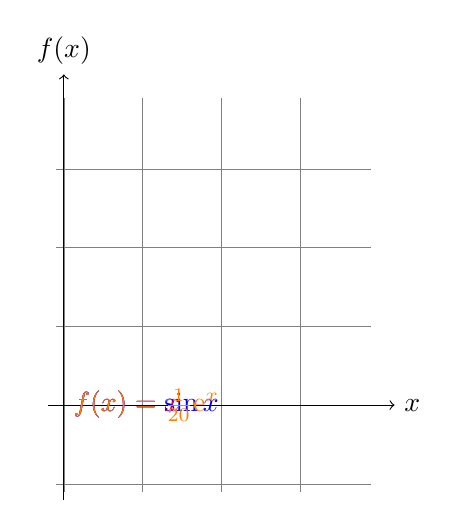
\begin{tikzpicture}[domain=0:4]
    \draw[very thin,color=gray] (-0.1,-1.1) grid (3.9,3.9);
    \draw[->] (-0.2,0) -- (4.2,0) node[right] {$x$};
    \draw[->] (0,-1.2) -- (0,4.2) node[above] {$f(x)$};
    \draw[color=red] plot[id=x] function{x}
        node[right] {$f(x) =x$};
    \draw[color=blue] plot[id=sin] function{sin(x)}
        node[right] {$f(x) = \sin x$};
    \draw[color=orange] plot[id=exp] function{0.05*exp(x)}
        node[right] {$f(x) = \frac{1}{20} \mathrm e^x$};
\end{tikzpicture}
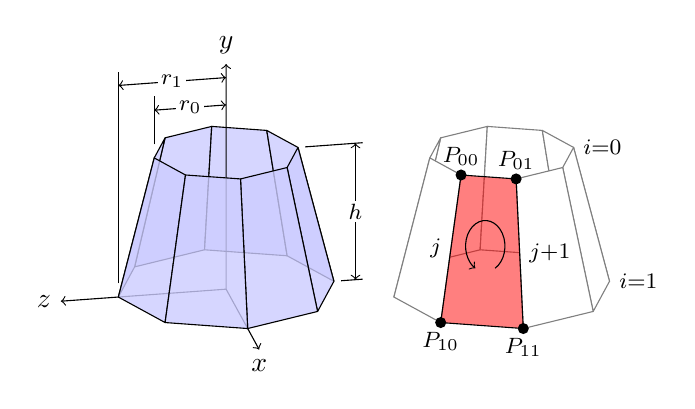
\begin{tikzpicture}[join=round]
    \tikzstyle{conefill} = [fill=blue!20,fill opacity=0.8]
    \tikzstyle{ann} = [fill=white,font=\footnotesize,inner sep=1pt]
    \tikzstyle{ghostfill} = [fill=white]
    \tikzstyle{ghostdraw} = [draw=black!50]
    \filldraw[conefill](-.775,1.922)--(-1.162,.283)--(-.274,.5)
                        --(-.183,2.067)--cycle;
    \filldraw[conefill](-.183,2.067)--(-.274,.5)--(.775,.424)
                        --(.516,2.016)--cycle;
    \filldraw[conefill](.516,2.016)--(.775,.424)--(1.369,.1)
                        --(.913,1.8)--cycle;
    \filldraw[conefill](-.913,1.667)--(-1.369,-.1)--(-1.162,.283)
                        --(-.775,1.922)--cycle;
    \draw(1.461,.107)--(1.734,.127);
    \draw[arrows=<->](1.643,1.853)--(1.643,.12);
    \filldraw[conefill](.913,1.8)--(1.369,.1)--(1.162,-.283)
                        --(.775,1.545)--cycle;
    \draw[arrows=->,line width=.4pt](.274,-.5)--(0,0)--(0,2.86);
    \draw[arrows=-,line width=.4pt](0,0)--(-1.369,-.1);
    \draw[arrows=->,line width=.4pt](-1.369,-.1)--(-2.1,-.153);
    \filldraw[conefill](-.516,1.45)--(-.775,-.424)--(-1.369,-.1)
                        --(-.913,1.667)--cycle;
    \draw(-1.369,.073)--(-1.369,2.76);
    \draw(1.004,1.807)--(1.734,1.86);
    \filldraw[conefill](.775,1.545)--(1.162,-.283)--(.274,-.5)
                        --(.183,1.4)--cycle;
    \draw[arrows=<->](0,2.34)--(-.913,2.273);
    \draw(-.913,1.84)--(-.913,2.447);
    \draw[arrows=<->](0,2.687)--(-1.369,2.587);
    \filldraw[conefill](.183,1.4)--(.274,-.5)--(-.775,-.424)
                        --(-.516,1.45)--cycle;
    \draw[arrows=<-,line width=.4pt](.42,-.767)--(.274,-.5);
    \node[ann] at (-.456,2.307) {$r_0$};
    \node[ann] at (-.685,2.637) {$r_1$};
    \node[ann] at (1.643,.987) {$h$};
    \path (.42,-.767) node[below] {$x$}
        (0,2.86) node[above] {$y$}
        (-2.1,-.153) node[left] {$z$};
    % Second version of the cone
    \begin{scope}[xshift=3.5cm]
    \filldraw[ghostdraw,ghostfill](-.775,1.922)--(-1.162,.283)--(-.274,.5)
                                   --(-.183,2.067)--cycle;
    \filldraw[ghostdraw,ghostfill](-.183,2.067)--(-.274,.5)--(.775,.424)
                                   --(.516,2.016)--cycle;
    \filldraw[ghostdraw,ghostfill](.516,2.016)--(.775,.424)--(1.369,.1)
                                   --(.913,1.8)--cycle;
    \filldraw[ghostdraw,ghostfill](-.913,1.667)--(-1.369,-.1)--(-1.162,.283)
                                   --(-.775,1.922)--cycle;
    \filldraw[ghostdraw,ghostfill](.913,1.8)--(1.369,.1)--(1.162,-.283)
                                   --(.775,1.545)--cycle;
    \filldraw[ghostdraw,ghostfill](-.516,1.45)--(-.775,-.424)--(-1.369,-.1)
                                   --(-.913,1.667)--cycle;
    \filldraw[ghostdraw,ghostfill](.775,1.545)--(1.162,-.283)--(.274,-.5)
                                   --(.183,1.4)--cycle;
    \filldraw[fill=red,fill opacity=0.5](-.516,1.45)--(-.775,-.424)--(.274,-.5)
                                         --(.183,1.4)--cycle;
    \fill(-.775,-.424) circle (2pt);
    \fill(.274,-.5) circle (2pt);
    \fill(-.516,1.45) circle (2pt);
    \fill(.183,1.4) circle (2pt);
    \path[font=\footnotesize]
            (.913,1.8) node[right] {$i\hbox{$=$}0$}
            (1.369,.1) node[right] {$i\hbox{$=$}1$};
    \path[font=\footnotesize]
            (-.645,.513) node[left] {$j$}
            (.228,.45) node[right] {$j\hbox{$+$}1$};
    \draw (-.209,.482)+(-60:.25) [yscale=1.3,->] arc(-60:240:.25);
    \fill[black,font=\footnotesize]
                    (-.516,1.45) node [above] {$P_{00}$}
                    (-.775,-.424) node [below] {$P_{10}$}
                    (.183,1.4) node [above] {$P_{01}$}
                    (.274,-.5) node [below] {$P_{11}$};
    \end{scope}
\end{tikzpicture}

Рассказывать о возможностях я не буду, их слишком много. Тем более, что по TikZ есть отличный мануал. Есть дополнительный супер-пакет \verb'TikZ-2d'. Специально для рисунков по геометрии. Для него Вы тоже без труда найдёте мануал в интернет.

Чтобы добавить пакет, нужно сказать в преамбуле \verb'\usepackage{tikz}\usetikzlibrary{calc}'.

Расскажу про тонкость. Можно рисовать графики функций. Для этого нужно дополнительно установить \verb'gnuplot'. Если Вы собираетесь его использовать, то не забудьте добавить в первую строчку файла
\verb'%& -shell-escape'.

Для вставки уже подготовленных рисунков можно использовать команду:
\begin{verbatim}
  \putthere{103mm}{-10mm}{%
      \begin{tikzpicture}
          . . .
      \end{tizpicture}}
      {7cm}{\risn Пятиугольные числа.}
\end{verbatim}
Первый параметр --- смещение по горизонтали, второй --- по вертикали, третий --- сам рисунок, четвёртый --- ширина подписи, пятый --- сама подпись (при этом команда \verb'risn' вставляет \fbox{\risn}).


\newpage
Рисунки вставляются так:
\putthere{103mm}{-10mm}{%
    %
    % Картинка для пятиугольных чисел
    %
      \begin{tikzpicture}
      [scale=.11
      ,ver/.style={circle,draw=blue!50,fill=blue!20,thick,inner sep=0,minimum size=3}
      ,lin/.style={color=blue!80}]
        \coordinate (A0) at (0,0);
        \coordinate (A1) at (7,0);
        \coordinate (A2) at (20,0);
        \coordinate (A3) at (42,0);
        \node[ver] at (A0){};
        \draw[lin,very thin] (A1) + (-126:4) -- +(18:4);
        \draw[lin,very thin] (A1) + (-126:4) -- +(90:4);
        \foreach \angle in {18,90,...,306}{
          \draw[lin] (A1)
                                       +(\angle:4)    node[ver]{}
                                    -- +(\angle+72:4);
        }
        \draw[lin,very thin] (A2) + (-126:8) -- +(18:8);
        \draw[lin,very thin] (A2) + (-126:8) -- +(90:8);
        \foreach \angle in {18,90,...,306}{
          \draw[lin] (A2)
                                       +(\angle:8)    node[ver]{} coordinate (A)
                                    -- +(\angle+72:8)             coordinate (B);
          \node[ver] at  ($ (A)!.5!(B) $){};
          \draw[lin] (A2) ++ (-126:8) ++ (54:4)
                                       +(\angle:4)    node[ver]{} coordinate (A)
                                    -- +(\angle+72:4)             coordinate (B);
        }
        \draw[lin,very thin] (A3) + (-126:12) -- +(18:12);
        \draw[lin,very thin] (A3) + (-126:12) -- +(90:12);
        \foreach \angle in {18,90,...,306}{
          \draw[lin] (A3)
                                       +(\angle:12)    node[ver]{} coordinate (A)
                                    -- +(\angle+72:12)             coordinate (B);
          \node[ver] at  ($ (A)!.333!(B) $){};
          \node[ver] at  ($ (A)!.666!(B) $){};
          \draw[lin] (A3) ++ (-126:12) ++ (54:8)
                                       +(\angle:8)    node[ver]{} coordinate (A)
                                    -- +(\angle+72:8)             coordinate (B);
          \node[ver] at  ($ (A)!.5!(B) $){};
          \draw[lin] (A3) ++ (-126:12) ++ (54:4)
                                       +(\angle:4)    node[ver]{} coordinate (A)
                                    -- +(\angle+72:4)             coordinate (B);
        }
      \end{tikzpicture}
}{7cm}{\risn Пятиугольные числа.}

\begin{verbatim}
  \putthere{163mm}{-9mm}{%
    %
    % Картинка для пятиугольных чисел
    %
      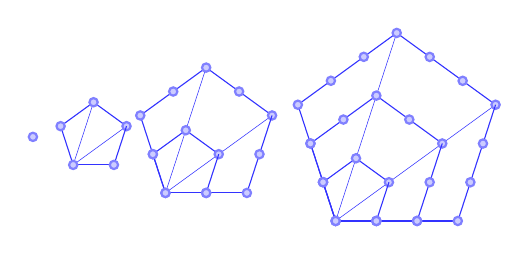
\begin{tikzpicture}
      [scale=.11
      ,ver/.style={circle,draw=blue!50,fill=blue!20,thick,inner sep=0,minimum size=3}
      ,lin/.style={color=blue!80}]
        \coordinate (A0) at (0,0);
        \coordinate (A1) at (7,0);
        \coordinate (A2) at (20,0);
        \coordinate (A3) at (42,0);
        \node[ver] at (A0){};
        \draw[lin,very thin] (A1) + (-126:4) -- +(18:4);
        \draw[lin,very thin] (A1) + (-126:4) -- +(90:4);
        \foreach \angle in {18,90,...,306}{
          \draw[lin] (A1)
                                       +(\angle:4)    node[ver]{}
                                    -- +(\angle+72:4);
        }
        \draw[lin,very thin] (A2) + (-126:8) -- +(18:8);
        \draw[lin,very thin] (A2) + (-126:8) -- +(90:8);
        \foreach \angle in {18,90,...,306}{
          \draw[lin] (A2)
                                       +(\angle:8)    node[ver]{} coordinate (A)
                                    -- +(\angle+72:8)             coordinate (B);
          \node[ver] at  ($ (A)!.5!(B) $){};
          \draw[lin] (A2) ++ (-126:8) ++ (54:4)
                                       +(\angle:4)    node[ver]{} coordinate (A)
                                    -- +(\angle+72:4)             coordinate (B);
        }
        \draw[lin,very thin] (A3) + (-126:12) -- +(18:12);
        \draw[lin,very thin] (A3) + (-126:12) -- +(90:12);
        \foreach \angle in {18,90,...,306}{
          \draw[lin] (A3)
                                       +(\angle:12)    node[ver]{} coordinate (A)
                                    -- +(\angle+72:12)             coordinate (B);
          \node[ver] at  ($ (A)!.333!(B) $){};
          \node[ver] at  ($ (A)!.666!(B) $){};
          \draw[lin] (A3) ++ (-126:12) ++ (54:8)
                                       +(\angle:8)    node[ver]{} coordinate (A)
                                    -- +(\angle+72:8)             coordinate (B);
          \node[ver] at  ($ (A)!.5!(B) $){};
          \draw[lin] (A3) ++ (-126:12) ++ (54:4)
                                       +(\angle:4)    node[ver]{} coordinate (A)
                                    -- +(\angle+72:4)             coordinate (B);
        }
      \end{tikzpicture}
}{7cm}{\risn Пятиугольные числа.}

\end{verbatim}

Как делать простые рисунки --- мне писать лень. Мануал действительно довольно хороший. Есть некоторые тонкости. Если хочется про них узнать --- спросите у меня лично.

\newpage
\section{Сокращения от DMVN}

\subsection{Операторы}
\begin{center}
\begin{tabular}{|c|c|c||c|c|c|}
\hline \textbf{Команда} & \textbf{Оператор} & \textbf{Описание}&
\textbf{Команда} & \textbf{Оператор} & \textbf{Описание}  \\
\hline \verb'\Ad'  & $\Ad$  &   Присоединённый оператор & \verb'\ad' & $\ad$ & Присоединённый операток  \\
\hline \verb'\CoAd'  & $\CoAd$  &   Коприсоединённый оператор & \verb'\coad'  & $\coad$  &   Коприсоединённый оператор \\
\hline \verb'\Arg' & $\Arg$ &   Аргумент  & \verb'\area' & $\area$ & Площадь    \\
\hline \verb'\arsh' & $\arsh$ & Ареа\д синус  & \verb'\Aut' & $\Aut$ &  Автоморфизмы \\
\hline \verb'\Card' & $\Card$ & Мощность множества&\verb'\Char' &$\Char$& Характеристика поля  \\
\hline \verb'\Cl' & $\Cl$ &   Замыкание & \verb'\codim' & $\codim$ & Коразмерность    \\
\hline \verb'\Coim' & $\Coim$ & Прообраз & \verb'\Com' & $\Com$ & Вычислимые функции    \\
\hline \verb'\const' & $\const$ & Константа  &\verb'\conv' & $\conv$ & Выпуклая оболочка    \\
\hline \verb'\Corr' & $\Corr$ &  Корреляция & \verb'\cov' & $\cov$ &   Ковариация  \\
\hline \verb'\diag' & $\diag$ & Диагональная матрица & \verb'\diam' & $\diam$ &  Диаметр   \\
\hline \verb'\dist' & $\dist$ &  Расстояние & \verb'\Div' & $\Div$ &   Дивергенция  \\
\hline \verb'\Dom' & $\Dom$ &Область определения &\verb'\dom' & $\dom$ &   Область определения  \\
\hline \verb'\End' & $\End$ & Группа эндоморфизмов &\verb'\epig' & $\epig$ &  Надграфик \\
\hline \verb'\extr' & $\extr$ &  Экстремум &\verb'\grad' & $\grad$ & Градиент    \\
\hline \verb'\Graph' & $\Graph$ & График & \verb'\GCD' & $\GCD$ & Наибольший общий делитель \\
\hline\verb'\Hom'&$\Hom$&Пространство гомоморфизмов&\verb'\id'&$\id$&Тождественное отображение \\
\hline \verb'\Im' & $\Im$ &  Образ или мнимая часть&\verb'\Img'&$\Img$ &  Образ или мнимая часть\\
\hline \verb'\ind' & $\ind$ &  Индекс векторного поля &\verb'\Int' & $\Int$ &  Внутренность \\
\hline \verb'\Inn' & $\Inn$ &  Внутренние автоморфизмы&\verb'\Isom'& $\Isom$ & Группа изометрий \\
\hline \verb'\Ker' & $\Ker$ &  Ядро &\verb'\Law' & $\Law$ &  Закон распределения \\
\hline\verb'\LCM'&$\LCM$&Наименьшее общее кратное&\verb'\Lin'&$\Lin$&Пространство линейных отображений\\
\hline \verb'\Ln' & $\Ln$ &  Логарифм &\verb'\mes' & $\mes$ &  Мера Лебега \\
\hline \verb'\Mat' & $\Mat$ &  Множество матриц &\verb'\Orb' & $\Orb$ &  Орбита \\
\hline \verb'\ord' & $\ord$ &  Порядок &\verb'\Out' & $\Out$ &  Внешние автоморфизмы   \\
\hline \verb'\Pin' & $\Pin$ &  Пинорная группа  &\verb'\Prj' & $\Prj$ &  Проекция   \\
\hline \verb'\Quot' & $\Quot$ &  Поле отношений &\verb'\Ran' & $\Ran$ &   Образ отображения \\
\hline \verb'\Re' & $\Re$ &   Вещественная часть &\verb'\Rea' & $\Rea$ &   Вещественная часть \\
\hline \verb'\res' & $\res$ &   Вычет$^*$ &\verb'\rk' & $\rk$ &   Ранг \\
\hline \verb'\rot' & $\rot$ & Ротор &\verb'\sgn' & $\sgn$ & Знак \\
\hline \verb'\Si' & $\Si$ &  Интегральный синус &\verb'\Spec' & $\Spec$ &  Спектр \\
\hline \verb'\Spin' & $\Spin$ &  Спинорная группа & \verb'\St' & $\St$ &  Стабилизатор \\
\hline \verb'\supp' & $\supp$ &  Носитель &\verb'\Tor' & $\Tor$ & Подгруппа кручения \\
\hline \verb'\tr' & $\tr$ &  След &\verb'\vp' & $\vp$ &  Главное значение \\
\hline \verb'\Var' & $\Var$ &  Полное изменение (вариация)& \verb'\Ann' & $\Ann$ & Аннулятор   \\
\hline
\end{tabular}
\end{center}

Звёздочками отмечены команды, в которых использование команды \verb'\limits'
поставит индекс под значком, а не справа от него.

\subsection{Команды, заменяющие окружения}

\subsubsection{Матрицы}

\begin{center}
\begin{tabular}{cccc}
\rulezz\verb"\mat": $\mat{a&b\\c&d}$ &
\verb"\rbmat": $\rbmat{a&b\\c&d}$ &
\verb"\sbmat": $\sbmat{a&b\\c&d}$ &
\verb"\cbmat": $\cbmat{a&b\\c&d}$ \\
\rulezz\verb"\mbmat": $\mbmat{a&b\\c&d}$ &
\verb"\nbmat": $\nbmat{a&b\\c&d}$ &
\verb"\rcmat": $\rcmat{a&b\\c&d}$ &
\verb"\lcmat": $\lcmat{a&b\\c&d}$
\end{tabular}
\end{center}

\subsubsection{Прочие команды\д окружения}

\begin{items}{-1}

\item Таблица \verb"\tab": \tab{|c|c|}{\hline A&B \\ \hline a&b\\ \hline}\т
\verb'\tab{|c|c|}{\hline A&B \\ \hline a&b \\ \hline}'

\item Таблица, выровненная по центру: \verb"\ctab": \ctab{|c|c|}{\hline A & B\\\hline a & b\\\hline}
\item Фигурная скобка \verb"\case": $\Dc(x) := \case{1, & x\in\Q,\\0, & x\notin \Q.}$ Именно так определяется функция Дирихле.
\begin{verbatim}
$\Dc(x) := \case{1, & x\in\Q,\\0, & x\notin \Q.}$
\end{verbatim}

\item Фигурная скобка \verb"\bcase" для больших формул . Почувствуйте разницу.
Слева \verb"\case", справа \verb"\bcase":

$$
\case{
m_i r_i= \suml{\al=1}{a}\la_{\al}\pf{f_{\al}}{r_i}+\suml{\be=1}{b}\mu_{\be}b_{\be i},\\
f_{\al}(r,t)=0,\\
\ph_{\be}:=\suml{i=1}{n}b_{\be i}(r,t)r_i+b_{\be}(r,t)=0.
}
\bcase{
&m_i r_i = \suml{\al=1}{a}\la_{\al}\pf{f_{\al}}{r_i}+\suml{\be=1}{b}\mu_{\be}b_{\be i},\\
&f_{\al}(r,t)=0,\\
&\ph_{\be}:=\suml{i=1}{n}b_{\be i}(r,t)r_i+b_{\be}(r,t)=0.}
$$
В этой команде используется окружение \texttt{aligned}. Для выравнивания по левому краю в начале каждой строки нужно ставить \texttt{\&}.
Отличие, конечно, состоит в присутствии \texttt{displaymath}.
Использование команды таково:
\begin{verbatim}
$$
\bcase{
Большая формула номер раз \\
Большая формула номер два \\
Большая формула номер три
}
$$
\end{verbatim}


\item Центрирование текста \verb"\cent": \cent{Этот текст расположен в центре строки.}

\item Уравнение с~номером \eqn{x+y=z}
делается так: \verb'\eqn{x+y=z}'.

\item Уравнение без номера \equ{x+y=z}
делается так: \verb'\equ{x+y=z}'.

\item Система уравнений с \verb"\bcase" \eqb{\dot q &= \phm\pf{H}{p},\\ \dot p &= -\pf{H}{q}.}
делается так: \verb'\eqb{\dot q = \phm\pf{H}{p},\\ \dot p &= -\pf{H}{q}.}'.

\item Уравнение со звёздочкой вместо номера \eqa{*}{x+y=z}
делается так: \verb'\eqa{*}{x+y=z}'.
При этом внутренний счётчик \verb'equation' увеличивается на единицу, так что следующее нумерованное
уравнение \eqn{x+y=z} будет иметь номер \arabic{equation},\addtocounter{equation}{-1} а~не~\arabic{equation}.
\addtocounter{equation}{1}

\item Окружения \verb'multline' и~\verb'multline*' заменяют обёртки \verb'\mln' и~\verb'\ml'
соответственно. Ещё имеется команда \verb'\mla', которая работает так же, как и \verb'\eqa'.
\end{items}

\subsection{Нумерация, списки, пункты и подпункты}

\subsubsection{Окружение для нумерации \emph{nums}}

\begin{nums}{-3}
\item При использовании \verb'enumerate' расстояние между строками получается очень большим
\item Окружение \verb'nums' имеет один обязательный параметр. Это число, определяющее
то количество пунктов, в~которое будет установлена переменная \verb'\itemsep'.
Если указано отрицательное число, то стандартное расстояние уменьшится
в~указанное число пунктов.
\end{nums}

\subsubsection{Окружение для списков \emph{items}}

\begin{items}{-3}
\item При использовании \verb'itemize' расстояние между строками получается очень большим
\item Окружение \verb'items' имеет один обязательный параметр. Это число, определяющее
то количество пунктов, в~которое будет установлена переменная \verb'\itemsep'.
Если указано отрицательное число, то стандартное расстояние уменьшится
в~указанное число пунктов.
\end{items}

\subsection{Картинки и всё такое прочее}

\subsubsection{Команды для вставки плавающих объектов}


% \dmvnpiclh{mmlogo3.pdf}{2}
% Однако эти команды на данный момент признаны авторами устаревшими. Мы не рекомендуем
% их использовать. Очередная\dmvnpicl{mmlogo3.pdf}{1} разработка\т команды \verb'\dmvnpicl' и~\verb'\dmvnpicr',
% а~также их аналоги, предусматривающие возможность двигать изображение по вертикали\т
% команды \verb'\dmvnpicla' и~\verb'\dmvnpicra'. Здесь буква \verb'a'\т начало слова \emph{adjust}.
% Для управления отступами используются команды \verb'\dmvnpiclh' и~\verb'\dmvnpicrh'\т соответственно
% левый и~правый отступ. Картинка будет вставлена в~текст после той строки, где случилась
% команда вставки картинки. Команду управления отступом нужно писать до начала абзаца.
% В~этот абзац картинка была вставлена так: в~начале абзаца прописано
% \begin{verbatim}
%              \dmvnpiclh{mmlogo3}{2}
%              Однако эти команды на данный момент признаны...
% \end{verbatim}
% Команда вставки картинки находится во второй строке:
% \begin{verbatim}
% ... их использовать. Очередная\dmvnpicl{mmlogo3}{1} разработка ...
% \end{verbatim}
%
% Теперь разберём аргументы команд отступа. Первый аргумент\т это имя файла с~картинкой,
% а~второй\т число, которое устанавливает параметр \verb'\hangafter'. Что это такое\т читайте
% \TeX book. Что касается аргументов команд вставки картинки, то первый аргумент\т это опять\д таки
% имя файла, а~второй\т номер рисунка. Команды, предусматривающие движение по вертикали,
% имеют третий аргумент, который определяет величину сдвига в~любых допустимых \TeX нических единицах.
% Например, если нас не устраивает слишком большой отступ сверху, можно подправить команду так:
% \begin{verbatim}
% ... их использовать. Очередная\dmvnpicla{mmlogo3}{1}{-.5pc} разработка ...
% \end{verbatim}



\subsection{Шрифты и значки}

\subsubsection{Буквы}

\verb'\db \ib \jb \kb \nb \rb': $\db\; \ib\; \jb\; \kb\; \nb\; \rb$.

\verb$\Ac,\Bc,\Cc:$ $\Ac\Bc\Cc\Dc\Ec\Fc\Gc\Hc\Ic\Jc\Kc\Lc\Mc\Nc\Oc\Pc\Qc\Rc\Sc\Tc\Uc\Vc\Wc\Xc\Yc\Zc$.

\verb$\Ab,\Bb,\Cb:$ $\Ab\Bb\Cb\Db\Eb\Fb\Gb\Hb\Ib\Jb\Kb\Lb\Mb\Nb\Ob\Pb\Qb\Rb\Sb\Tb\Ub\Vb\Wb\Xb\Yb\Zb$.

\verb$\As,\Bs,\Cs:$ $\As\Bs\Cs\Ds\Es\Fs\Gs\Hs\Is\Js\Ks\Ls\Ms\Ns\Os\Ps\Qs\Rs\Ss\Ts\Us\Vs\Ws\Xs\Ys\Zs$.

\verb$\Af,\Bf,\Cf:$ $\Af\Bf\Cf\Df\Ef\Ff\Gf\Hf\If\Jf\Kf\Lf\Mf\Nf\Of\Pf\Qf\Rf\Sf\Tf\Uf\Vf\Wf\Xf\Yf\Zf$.

\verb$\Ag,\Bg,\Cg:$ $\Ag\Bg\Cg\Dg\Eg\Fg\Gg\Hg\Ig\Jg\Kg\Lg\Mg\Ng\Og\Pg\Qg\Rg\Sg\Tg\Ug\Vg\Wg\Xg\Yg\Zg$.

\verb$\A \B \F \K \N \Q \R \T \Z \Cbb \Ebb \Hbb \Ibb \Lbb \Sbb$:
$\quad\A\;\B\;\F\;\K\;\N\;\Q\;\R\;\T\;\Z\;\Cbb\;\Ebb\;\Hbb\;\Ibb\;\Lbb\;\Sbb$.

\subsubsection{Значки}

\verb$\GA \GL \PSL \SO \SU \SL \Sp \UT \ggt \hgt \glg \slg \sog \spg$:

$\quad\GA\;\GL\;\PGL\;\PSL\;\SO\;\SU\;\SL\;\Sp\;\UT\;\ggt\;\hgt\;\glg\;\slg\;\sog\;\spg$.

\medskip


\subsubsection{Греческие буквы}
\begin{center}
\begin{tabular}{|c|c|c||c|c|c|}
\hline \textbf{Новая} & \textbf{Обычная} & \textbf{Символ} &
\textbf{Новая} & \textbf{Старая} & \textbf{Символ} \\
\hline \verb$\al$ & \verb$\alpha$ & $\al$ &      \verb$\be$ & \verb$\beta$ & $\be$ \\
\hline \verb$\Be$ & \verb$\textrm{B}$ & $\Be$ &  \verb$\ga$ & \verb$\gamma$ & $\ga$ \\
\hline \verb$\Ga$ & \verb$\Gamma$ & $\Ga$ &      \verb$\de$ & \verb$\delta$ & $\de$ \\
\hline \verb$\De$ & \verb$\Delta$ & $\De$ &      \verb$\ep$ & \verb$\varepsilon$ & $\ep$\\
\hline \verb$\ka$ & \verb$\varkappa$ & $\ka$ &   \verb$\la$ & \verb$\lambda$ & $\la$ \\
\hline \verb$\La$ & \verb$\Lambda$ & $\La$ &     \verb$\si$ & \verb$\sigma$ & $\si$ \\
\hline \verb$\Sig$ & \verb$\Sigma$ & $\Sig$ &    \verb$\om$ & \verb$\omega$ & $\om$ \\
\hline \verb$\Om$ & \verb$\Omega$ & $\Om$  &     \verb$\ph$ & \verb$\varphi$ & $\ph$ \\
\hline \verb$\Ph$ & \verb$\Phi$ & $\Ph$  & \verb$\rh$ & \verb$\rho$ & $\rh$ \\
\hline \verb$\ta$ & \verb$\theta$ & $\ta$ & \verb$\Ta$ & \verb$\Theta$ & $\Ta$ \\
\hline \verb$\ze$ & \verb$\zeta$ & $\ze$ & \verb$\nab$ & \verb$\nabla$ & $\nab$ \\
\hline
\end{tabular}
\end{center}

\subsection{Скобки: сделайте их больше, Больше, БОЛЬШЕ!}
Команды работают так: \verb"\команда{формула в скобках}".
\begin{center}
\begin{tabular}{ccc}
\verb"\hr,\br,\Br,\bbr,\bbbr" & Круглые & $\hr{\suml{a}{b}}$, $\br{a}$, $\Br{a}$, $\bbr{a}$, $\bbbr{a}$ \\
\verb"\hs,\bs,\BS,\bbs,\bbbs" & Квадратные & $\hs{\suml{a}{b}}$, $\bs{a}$, $\BS{a}$, $\bbs{a}$, $\bbbs{a}$ \\
\verb"\hsr,\bsr,\Bsr,\bbsr,\bbbsr" & Правый полуинтервал & $\hsr{\suml{a}{b}}$, $\bsr{a}$, $\Bsr{a}$, $\bbsr{a}$, $\bbbsr{a}$ \\
\verb"\hrs,\brs,\Brs,\bbrs,\bbbrs" & Левый полуинтервал & $\hrs{\suml{a}{b}}$, $\brs{a}$, $\Brs{a}$, $\bbrs{a}$, $\bbbrs{a}$ \\
\verb"\hm,\bm,\Bm,\bbm,\bbbm" & Модуль & $\hm{\suml{a}{b}}$, $\bm{a}$, $\Bm{a}$, $\bbm{a}$, $\bbbm{a}$ \\
\verb"\hc,\bc,\BC,\bbc,\bbbc" & Фигурные & $\hc{\suml{a}{b}}$, $\bc{a}$, $\BC{a}$, $\bbc{a}$, $\bbbc{a}$ \\
\verb"\hn,\bn,\Bn,\bbn,\bbbn" & Норма & $\hn{\suml{a}{b}}$, $\bn{a}$, $\Bn{a}$, $\bbn{a}$, $\bbbn{a}$ \\
\verb"\ha,\ba,\Ba,\bba,\bbba" & Угловые & $\ha{\suml{a}{b}}$, $\ba{a}$, $\Ba{a}$, $\bba{a}$, $\bbba{a}$ \\
\verb"\hfl,\bfl,\Bfl,\bbfl,\bbbfl" & Нижние & $\hfl{\suml{a}{b}}$, $\bfl{a}$, $\Bfl{a}$, $\bbfl{a}$, $\bbbfl{a}$ \\
\verb"\hce,\bce,\Bce,\bbce,\bbbce" & Верхние & $\hce{\suml{a}{b}}$, $\bce{a}$, $\Bce{a}$, $\bbce{a}$, $\bbbce{a}$ \\
\end{tabular}
\end{center}

Чтобы не думать, какой высоты скобки нужно ставить в~сложных выражениях типа
$$
  \hs{\sqrt{\hr{\frac 1n + n}^n} + \hc{\frac{\sqrt{n}}{2}}^2},
$$
их лучше сразу делать выровненными: \verb'\hs{\sqrt{\hr{\frac 1n + n}^n} + \hc{\frac{\sqrt n}{2}}^2}'.


\subsection{<<Пусть $\la_1$, и так далее, $\la_2$\т собственные значения\ldots>>}
\begin{center}
\begin{tabular}{|c|c|c||c|c|c|}
\hline \textbf{Команда} & \textbf{Назначение} & \textbf{Вид} & \textbf{Команда} & \textbf{Назначение} & \textbf{Вид} \\
\hline \verb$\sco$ & Запятые & $a_1\sco a_n$ & \verb$\spl$ & Сумма & $a_1\spl a_n$ \\
\hline \verb$\sd$ & Произведение & $a_1\sd a_n$ & \verb$\st$ & Прямое произведение & $G_1\st G_n$ \\
\hline \verb$\sop$ & Прямая сумма & $G_1\sop G_n$ & \verb$\sot$ & Тензорное произведение & $V_1\sot V_n$ \\
\hline \verb$\sw$ & Внешнее произведение & $dx_1 \sw dx_n$ &  \verb'\sa' & Конъюнкция & $A_1\sa A_n$\\
\hline \verb$\sle$ & По возрастанию & $a_1 \sle a_n$ &  \verb'\sge' & По убыванию & $a_1\sge a_n$\\
\hline \verb$\sles$ & Строго по возрастанию & $a_1 \sles a_n$ &  \verb'\sgre' & Строго по убыванию & $a_1\sgre a_n$\\
\hline
\end{tabular}
\end{center}
Кроме того, имеется команда \verb'\etc', которая означает <<$\etc$>>.



\subsection{Математические операции с <<пределами>>}

\subsubsection{Пределы и Интегралы}


\hbox to \textwidth{\hfil
\begin{tabular}{|c|c|}
\hline\rulez\verb'\intl[2]' & $ \intl{a}{b}f(x)\,dx$ \\
\hline\rulez\verb'\ints[1]' & $ \ints{A}f(x)\,dx$ \\
\hline\rulez\verb'\iints[1]' & $ \iints{A}f(x,y)\,dx\,dy$ \\
\hline
\end{tabular}\hfil
\begin{tabular}{|c|c|}
\hline\rulez\verb'\iiints[1]' & $ \iiints{A}f(x,y,z)\,dx\,dy\,dz$ \\
\hline\rulez\verb'\idotsints[1]' & $ \idotsints{A}f(x)\,dx$ \\
\hline\rulez\verb'\oints[1]' & $ \oints{A}f(x,y)\,dx\,dy$ \\
\hline
\end{tabular}\hfil
\begin{tabular}{|c|c|}
\hline\rulez\verb'\limn' & $\limn x_i$ \\
\hline\rulez\verb'\limx[1]' & $\limx{7} \dfrac{1}{x-7}$ \\
\hline
\end{tabular}
}\medskip


\subsubsection{Суммы}

$\suml{n=1}{\bes}\frac1n$ делается, например так: \verb"$\suml{n=1}{\bes}\frac1n$", или так:
\verb"$\sumnui\frac1n$".

\hbox to \textwidth{\hfil
\begin{tabular}{|c|c|}
\hline\rulez\verb'\suml[2]' & $\suml{i=j}{k}a_i$ \\
\hline\rulez\verb'\sums[1]' & $\sums{i \in I}$ \\
\hline\rulez\verb'\sumkui' & $\sumkui$ \\
\hline\rulez\verb'\sumnui' & $\sumnui$ \\
\hline\rulez\verb'\sumiui' & $\sumiui$ \\
\hline\rulez\verb'\sumkzi' & $\sumkzi$ \\
\hline
\end{tabular}\hfil
\begin{tabular}{|c|c|}
\hline\rulez\verb'\sumnzi' & $\sumnzi$ \\
\hline\rulez\verb'\sumizi' & $\sumizi$ \\
\hline\rulez\verb'\sumkun' & $\sumkun$ \\
\hline\rulez\verb'\sumiun' & $\sumiun$ \\
\hline\rulez\verb'\sumkzn' & $\sumkzn$ \\
\hline\rulez\verb'\sumizn' & $\sumizn$ \\
\hline
\end{tabular}\hfil
\begin{tabular}{|c|c|}
\hline\rulez\verb'\sumkum' & $\sumkum$ \\
\hline\rulez\verb'\sumium' & $\sumium$ \\
\hline\rulez\verb'\sumkzm' & $\sumkzm$ \\
\hline\rulez\verb'\sumizm' & $\sumizm$ \\
\hline\rulez\verb'\sumun' & $\sumun$ \\
\hline\rulez\verb'\sumzn' & $\sumzn$ \\
\hline
\end{tabular}\hfil
\begin{tabular}{|c|c|}
\hline\rulez\verb'\sumui' & $\sumui$ \\
\hline\rulez\verb'\sumzi' & $\sumzi$ \\
\hline\rulez\verb'\sumn' & $\sumn$ \\
\hline\rulez\verb'\sumi' & $\sumi$ \\
\hline
\end{tabular}\hfil}\medskip

\subsubsection{Произведения, пределы и прочее}

\hbox to \textwidth{\hfil
\begin{tabular}{|c|c|}
\hline\rulez\verb'\oplusl[2]' & $ \oplusl{i=1}{n}V_i$ \\
\hline\rulez\verb'\otimesl[2]' & $ \otimesl{i=1}{n}V_i$ \\
\hline\rulez\verb'\opluss[1]' & $ \opluss{i \in I}V_i$ \\
\hline\rulez\verb'\otimess[1]' & $ \otimess{i \in I}V_i$ \\
\hline\rulez\verb'\prodl[2]' & $ \prodl{i=j}{k}p_i$ \\
\hline
\end{tabular}\hfil
\begin{tabular}{|c|c|}
\hline\rulez\verb'\prods[1]' & $ \prods{i \in I}p_i$ \\
\hline\rulez\verb'\liml[1]' & $ \liml{n\ra\infty} x_n$ \\
\hline\rulez\verb'\ampl[2]' & $ \ampl{i=1}{n} A_i $ \\
\hline\rulez\verb'\amps[1]' & $ \amps{i\neq j} (x_i=x_j)$ \\
\hline\rulez\verb'\Varl[1]' & $ \Varl{\ga}$ \\
\hline
\end{tabular}\hfil
\begin{tabular}{|c|c|}
\hline\rulez\verb'\infl[1]' & $ \infl{i \in I}p_i$ \\
\hline\rulez\verb'\supl[1]' & $ \supl{i \in I}p_i$ \\
\hline\rulez\verb'\maxl[1]' & $ \maxl{i \in I}p_i$ \\
\hline\rulez\verb'\minl[1]' & $ \minl{i \in I}p_i$ \\
\hline\rulez\verb'\uliml[1]' & $ \uliml{i \in I}p_i$ \\
\hline\rulez\verb'\lliml[1]' & $ \lliml{i \in I}p_i$ \\
\hline
\end{tabular}\hfil}\medskip

\subsubsection{Объединения и пересечения}

\hbox to \textwidth{\hfil
\begin{tabular}{|c|c|}
\hline\rulez\verb'\cupl[2]' & $\cupl{i=j}{k}a_i$ \\
\hline\rulez\verb'\cups[1]' & $\cups{i \in I}$ \\
\hline\rulez\verb'\cupkui' & $\cupkui$ \\
\hline\rulez\verb'\cupnui' & $\cupnui$ \\
\hline\rulez\verb'\cupiui' & $\cupiui$ \\
\hline
\end{tabular}\hfil
\begin{tabular}{|c|c|}
\hline\rulez\verb'\cupkzi' & $\cupkzi$ \\
\hline\rulez\verb'\cupnzi' & $\cupnzi$ \\
\hline\rulez\verb'\cupizi' & $\cupizi$ \\
\hline\rulez\verb'\cupkun' & $\cupkun$ \\
\hline\rulez\verb'\cupiun' & $\cupiun$ \\
\hline
\end{tabular}\hfil
\begin{tabular}{|c|c|}
\hline\rulez\verb'\cupkzn' & $\cupkzn$ \\
\hline\rulez\verb'\cupizn' & $\cupizn$ \\
\hline\rulez\verb'\cupun' & $\cupun$ \\
\hline\rulez\verb'\cupzn' & $\cupzn$ \\
\hline\rulez\verb'\cupui' & $\cupui$ \\
\hline
\end{tabular}\hfil
\begin{tabular}{|c|c|}
\hline\rulez\verb'\cupzi' & $\cupzi$ \\
\hline\rulez\verb'\cupn' & $\cupn$ \\
\hline\rulez\verb'\cupi' & $\cupi$ \\
\hline\rulez\verb'\cupsql[2]' & $ \cupsql{i=1}{\bes}E_i$ \\
\hline\rulez\verb'\cupsqs[1]' & $ \cupsqs{i\in I}E_i$ \\
\hline
\end{tabular}\hfil}\medskip

\hbox to \textwidth{\hfil
\begin{tabular}{|c|c|}
\hline\rulez\verb'\capl[2]' & $\capl{i=j}{k}a_i$ \\
\hline\rulez\verb'\caps[1]' & $\caps{i \in I}$ \\
\hline\rulez\verb'\capkui' & $\capkui$ \\
\hline\rulez\verb'\capnui' & $\capnui$ \\
\hline\rulez\verb'\capiui' & $\capiui$ \\
\hline
\end{tabular}\hfil
\begin{tabular}{|c|c|}
\hline\rulez\verb'\capkzi' & $\capkzi$ \\
\hline\rulez\verb'\capnzi' & $\capnzi$ \\
\hline\rulez\verb'\capizi' & $\capizi$ \\
\hline\rulez\verb'\capkun' & $\capkun$ \\
\hline\rulez\verb'\capiun' & $\capiun$ \\
\hline
\end{tabular}\hfil
\begin{tabular}{|c|c|}
\hline\rulez\verb'\capkzn' & $\capkzn$ \\
\hline\rulez\verb'\capizn' & $\capizn$ \\
\hline\rulez\verb'\capun' & $\capun$ \\
\hline\rulez\verb'\capzn' & $\capzn$ \\
\hline\rulez\verb'\capui' & $\capui$ \\
\hline
\end{tabular}\hfil
\begin{tabular}{|c|c|}
\hline\rulez\verb'\capzi' & $\capzi$ \\
\hline\rulez\verb'\capn' & $\capn$ \\
\hline\rulez\verb'\capi' & $\capi$ \\
\hline
\end{tabular}\hfil}\medskip


\subsection{Часто употребляемые в математических текстах обозначения}

\subsubsection{Сокращения для стрелочек разного вида}

\begin{center}
\begin{tabular}{|c|c|c|}
\hline\verb'\to' & \verb'\rightarrow' & $a \to b$ \\
\hline\verb'\ra' & \verb'\rightarrow' &   $x_n \ra x$     \\
\hline\verb'\Ra' & \verb'\Rightarrow' &   $A\Ra B$     \\
\hline\verb'\nra' & \verb'\nrightarrow' &     $x_n \nra 0$   \\
\hline\verb'\longra' & \verb'\longrightarrow' &  $f_n \longra f$      \\
\hline\verb'\rra' & \verb'\rightrightarrows' &   $f_n \rra f$     \\
\hline\verb'\xra' & \verb'\xrightarrow' &      $f_n \xra{\mu} f$  \\
\hline\verb'\Lra' & \verb'\Leftrightarrow' &   $A \Lra B$     \\
\hline\verb'\lra' & \verb'\leftrightarrow' &    туда $\lra$ сюда    \\
\hline\verb'\ot' & \verb'\leftarrow' &   $x \ot x_n$     \\
\hline\verb'\ar' & \verb'\leftarrow' &  $x \ar x_n$      \\
\hline\verb'\lar' & \verb'\leftarrow' &  $x \lar x_n$      \\
\hline\verb'\Lar' & \verb'\Leftarrow' &   $B \Lar A$     \\
\hline\verb'\nla' & \verb'\nleftarrow' &    $x \nla x_n$    \\
\hline\verb'\longla' & \verb'\longleftarrow' &   $f \longla f_n$     \\
\hline\verb'\lla' & \verb'\leftleftarrows' &    $f \lla f_n$    \\
\hline\verb'\xla' & \verb'\xleftarrow' &     $f \xla{\nu} f_n$ \\
\hline\verb'\up' & \verb'\uparrow' &     $A_i \up A$   \\
\hline\verb'\inj' & \verb'\hookrightarrow' &     $K \inj L$   \\
\hline\verb'\map[1]' & \verb'\stackrel{#1}{\longrightarrow}' &  $A \map{f} B$      \\
\hline\verb'\corr[1]' & \verb'\stackrel{#1}{\longmapsto}' &     $g \corr{\ph} \ph(g)$   \\
\hline
\end{tabular}
\end{center}

\subsubsection{Сходимость, равенства \итп}

\begin{center}
\begin{tabular}{|c|c|c|c|}
\hline
\textbf{Команда} & \textbf{Пример} & \textbf{Вид} & \textbf{Описание} \\
\hline
\verb'\convu'   & \verb'f_n \convu{X} f'                   & $f_n \convu{X} f$ &      Равномерная сходимость      \\
\hline
\verb'\convs'  & \verb'A_n \convs A'                      & $A_n \convs A$ &    Сильная сходимость    \\
\hline
\verb'\convw'  & \verb'x_n \convw x'                      & $x_n \convw x$ &    Слабая сходимость    \\
\hline
\verb'\convws'  & \verb'x_n \convws x'                      & $x_n \convws x$ &    $*$-слабая сходимость    \\
\hline
\verb'\convas'  & \verb'\xi_n \convas \xi'                 & $\xi_n \convas \xi$ &    Сходимость почти наверное    \\
\hline
\verb'\convasu' & \verb'\xi_n \convasu \xi'                & $\xi_n \convasu \xi$ &   Монотонная сходимость п.н. \\
\hline
\verb'\convasl' & \verb'\xi_n \convasl \xi'                & $\xi_n \convasl \xi$ &   Монотонная сходимость п.н. \\
\hline
\verb'\convp'   & \verb'\xi_n \convp \xi'                  & $\xi_n \convp \xi$ &   Сходимость по вероятности \\
\hline
\verb'\convd'   & \verb'\xi_n \convd \xi'                  & $\xi_n \convd \xi$ &   Сходимость по распределению \\
\hline
\verb'\convae'  & \verb'f_n \convae f'                     & $f_n \convae f$ &  Сходимость почти всюду \\
\hline
\verb'\convaeu' & \verb'f_n \convaeu f'                    & $f_n \convaeu f$ &  Монотонная сходимость п.в. \\
\hline
\verb'\convael' & \verb'f_n \convael f'                    & $f_n \convael f$ &  Монотонная сходимость п.в. \\
\hline
\verb'\eqas'    & \verb'\xi \eqas \eta'                    & $\xi \eqas \eta$ &  Равенство почти наверное \\
\hline
\verb'\eqae'    & \verb'f \eqae g'                         & $f \eqae g$ &  Равенство почти всюду \\
\hline
\verb'\eqdef'   & \verb'Gx \eqdef \hc{g x \vl g \in G}'     & $Gx \eqdef \hc{gx \vl g \in G}$ &  Равенство по определению \\
\hline
\verb'\eqvl'    & \verb'\Ac\Bc v \eqvl{комм.}{20} \Bc\Ac v' & $\Ac\Bc v \eqvl{комм.}{20} \Bc\Ac v$ & Длинное равенство с надписью \\
\hline
\end{tabular}
\end{center}


\subsubsection{Прочие сокращения и новые определения}

\hbox to \textwidth{\hfil
\begin{tabular}{|c|c|c|}
\hline\rulez\verb'\ge'     & \verb'\geqslant'     & $a\ge b$   \\
\hline\rulez\verb'\le'     & \verb'\leqslant'     & $a\le b$   \\
\hline\rulez\verb'\nge'    & \verb'\ngeqslant'    & $a \nge b$     \\
\hline\rulez\verb'\nle'    & \verb'\nleqslant'    & $a \nle b$     \\
\hline\rulez\verb'\exi'    & \verb'\,\exists\,'   & $\exi x \in X$    \\
\hline\rulez\verb'\exu'    & \verb'\,\exists\,!\;'& $\exu x \in X$      \\
\hline\rulez\verb'\fa'     & \verb'\,\forall\,'   & $\fa \ep > 0$   \\
\hline\rulez\verb'\es'     & \verb'\varnothing'   & $\es$, а не $\emptyset$!   \\
\hline\rulez\verb'\bes'    & \verb'\infty'        & $\bes$ по\д русски    \\
\hline\rulez\verb'\pd'     & \verb'\partial'      & $\frac{\pd}{\pd ё}$     \\
\hline\rulez\verb'\subs'   & \verb'\subset'       & $A \subs B$     \\
\hline\rulez\verb'\sups'   & \verb'\supset'       & $B \sups A$    \\
\hline\rulez\verb'\subseq' & \verb'\subseteq'     & $A \subseq B$    \\
\hline\rulez\verb'\supseq' & \verb'\supseteq'     & $B \supseq A$   \\
\hline\rulez\verb'\wo'     & \verb'\smallsetminus'& $\R \wo \hc{0}$   \\
\hline\rulez\verb'\ol'     & \verb'\overline'     & $\ol x$   \\
\hline\rulez\verb'\os'     & \verb'\overset'      & $\os{\circ}{A}$    \\
\hline\rulez\verb'\us'     & \verb'\underset'     & $\us{\circ}{\forall}$    \\
\hline\rulez\verb'\ul'     & \verb'\underline'    & $\ul x$    \\
\hline\rulez\verb'\wh'     & \verb'\widehat'      & $x_1\sd \wh{x_i}\sd x_n$   \\
\hline\rulez\verb'\wt'     & \verb'\widetilde'    & $\wt{Y}$    \\
\hline\rulez\verb'\ub'     & \verb'\underbrace'   & $\ub{g^{-1} x g}$    \\
\hline\rulez\verb'\ob'     & \verb'\overbrace'    & $\ob{h_1 h_2}$    \\
\hline
\end{tabular}\hfil
\begin{tabular}{|c|c|c|}
\hline\rulez\verb'\cln'     & \verb'\colon'                & $f\cln\Cbb\ra\Cbb$    \\
\hline\rulez\verb'\wg'      & \verb'\wedge'                & $dx_1 \wg dx_2$   \\
\hline\rulez\verb'\ulim'    & \verb'\varlimsup'            & $\ulim$    \\
\hline\rulez\verb'\llim'    & \verb'\varliminf'            & $\llim$    \\
\hline\rulez\verb'\tri'     & \verb'\triangle'             & $\triangle$ \\
\hline\rulez\verb'\swo'     & \verb'\mathbin{\triangle}'   & $A \swo B$ \\
\hline\rulez\verb'\lhdp'    & \verb'\leftthreetimes'       & $\lhdp$       \\
\hline\rulez\verb'\rhdp'    & \verb'\rightthreetimes'      & $\rhdp$       \\
\hline\rulez\verb'\nl'      & \verb'\lhd'                  & $\nl$ \\
\hline\rulez\verb'\nr'      & \verb'\rhd'                  & $\nr$  \\
\hline\rulez\verb'\divs'    & \verb'\,\bigl\rvert\,'       & $m \divs n$     \\
\hline\rulez\verb'\ndivs'   & \verb'\!\nmid\!'             & $n \ndivs m$ \\
\hline\rulez\verb'\vl'      & \verb'\;\rvert\;'            & $\hc{g\in G \vl gx = x}$ \\
\hline\rulez\verb'\bvl'     & \verb'\;\big\rvert\;'        & $\bc{g \in G \bvl gx = x}$   \\
\hline\rulez\verb'\phm'     & \verb'\phantom{-}'           & $\rbmat{\phm a & b \\ -b & a}$ \\
\hline\rulez\verb'\factor[2]' & Смотрите исходник            & $\factor{G}{\Ker \ph} \cong \Img \ph$    \\
\hline\rulez\verb'\evu[3]'  & Смотрите исходник            & $u\evu{x=x_0}{9pt}{.6pc}$    \\
\hline\rulez\verb'\ev[2]'   & \verb'\evu{#1}{#2}{.65pc}}'  & $u\ev{x=x_0}{6pt}$    \\
\hline\rulez\verb'\evn[1]'  & \verb'\ev{#1}{10pt}'         & $A\evn{V}$    \\
\hline\rulez\verb'\usd[1]'  & \verb'\ol{\mathrm{S}}_{{#1}}'& $\usd{P}$  \\
\hline\rulez\verb'\lsd[1]'  & \verb'\ul{\mathrm{S}}_{{#1}}'& $\lsd{P}$   \\
\hline\rulez\verb'\pf[2]'   & \verb'\frac{\pd #1}{\pd #2}' & $\pf{ш}{щ}$  \\
\hline\rulez\verb'\dv'      & Смотрите исходник            & $a\dv b$ \\
\hline
\end{tabular}\hfil}\medskip

\end{document}
